\documentclass[aspectratio=169, 8 pt]{beamer}
\usepackage{pdfpages}
\usepackage{amsmath,amsthm,amssymb}
\usepackage{tikz}
\usepackage{pstricks}
\usepackage{ragged2e}
\usepackage{mathrsfs}
\usepackage{microtype}
\usepackage{bbm}
\usepackage{graphicx, wrapfig, subcaption, setspace, booktabs}
\usepackage{tabularx}
\usepackage{listings}
\usepackage{xcolor}
\usepackage{longtable}
%\usepackage{titlesec}
\usepackage{url, lipsum}
\usepackage{hyperref,bookmark}
\usepackage[T1]{fontenc}
\usepackage{amssymb}
\usepackage{tabularx}
\usepackage{listings}
\usepackage{xcolor}
\usepackage{longtable}
\usepackage{setspace}
\usepackage{float}
\usepackage{multirow}
\usepackage{tabularx}
\usepackage[at]{easylist}% easy lists with @ starting each item
\usepackage{algorithmic}
\usepackage{graphicx}
\usepackage{textcomp}
\usepackage{amsmath}
\usepackage[sc]{mathpazo}
\usepackage{datetime}
\usepackage{graphicx, wrapfig, subcaption, setspace, booktabs}
\usepackage[T1]{fontenc}
\usepackage{fourier}
\usepackage{url, lipsum}
\usepackage{hyperref,bookmark}
\usepackage[T1]{fontenc}
\usepackage{amssymb}
\usepackage{makecell, multirow, tabularx}
\usepackage{listings}
\usepackage[ruled,linesnumbered]{algorithm2e}

\usetheme{Pittsburgh}
\ifdefined\ishandout
	\usecolortheme{seagull}
\else
	\usecolortheme{scottybear}
\fi

\usefonttheme{serif}
\hypersetup{colorlinks,linkcolor=,urlcolor=links}

% Theorem Styles

\theoremstyle{theorem}
\newtheorem{thm}{Theorem}
\newtheorem{lm}{Lemma}
\newtheorem{ex}{Example}
\newtheorem{exs}{Examples}

\theoremstyle{definition}
\newtheorem{defn}{Definition}
\newtheorem{notation}{Notation}

\theoremstyle{remark}
\newtheorem*{remark}{Remark}

% Commands

\DeclareMathOperator{\diam}{diam}
\DeclareMathOperator{\id}{id}

\newcommand{\8}{\infty}
\newcommand{\A}{\mathscr{A}}
\newcommand{\C}{\mathbb{C}}
\newcommand{\N}{\mathbb{N}}
\newcommand{\Q}{\mathbb{Q}}
\newcommand{\R}{\mathbb{R}}
\newcommand{\Z}{\mathbb{Z}}
\newcommand{\iunit}{\mathbbm{i}}

\newcommand{\dif}{\mathrm{d}}
\newcommand{\diff}{\,\mathrm{d}}
\newcommand{\Dim}[1]{\dim_{\mathrm{#1}}}
\newcommand{\st}{\,|\,}
\newcommand{\ST}{\,\middle|\,}
\newcommand{\Poles}{\mathscr{P}}
\renewcommand\vec[1]{\boldsymbol{#1}}
\newcommand\Union{\mathop{\bigcup}}
\newcommand\Intersect{\mathop{\bigcap}}
\newcommand\union{\mathrel{\cup}}
\newcommand\intersect{\mathrel{\cap}}

\newgray{darkgrey}{.25}
\newgray{grey}{.5}
\newgray{lightgrey}{.75}
\newgray{vlightgrey}{.9}

\newcommand{\secslide}[2]{
	\section[#1]{#2}
		\begin{frame}
			\begin{center}
				\ifdefined\ishandout
					\textbf{\Huge\secname}
				\else
					\textcolor{structure}{\textbf{\Huge\secname}}
				\fi
			\end{center}
		\end{frame}
}

\renewcommand{\baselinestretch}{1.1}


\title[]{CO\textsubscript{2} and Cost Impacts of a Microgrid  with Electric Vehicle \\Charging Infrastructure: a Case Study in Southern California}
\author[]{Luis Fernando Enriquez-Contreras}
\institute[]{University of California, Riverside}
\date{January 9, 2024}


\definecolor{codegreen}{rgb}{0,0.6,0}
\definecolor{codegray}{rgb}{0.5,0.5,0.5}
\definecolor{codepurple}{rgb}{0.58,0,0.82}
\definecolor{backcolour}{rgb}{0.95,0.95,0.92}

\lstdefinestyle{mystyle}{
	backgroundcolor=\color{backcolour},   
	commentstyle=\color{codegreen},
	keywordstyle=\color{magenta},
	numberstyle=\tiny\color{codegray},
	stringstyle=\color{codepurple},
	basicstyle=\ttfamily\footnotesize,
	breakatwhitespace=false,         
	breaklines=true,                 
	captionpos=b,                    
	keepspaces=true,                 
	numbers=left,                    
	numbersep=5pt,                  
	showspaces=false,                
	showstringspaces=false,
	showtabs=false,                  
	tabsize=2
}

\lstset{style=mystyle}

\begin{document}

\usebackgroundtemplate{
	\tikz[overlay,remember picture] \node[opacity=0.04, at=(current page.center), yshift=-1.1in, xshift=1.75in] {
   
\includegraphics[height=3in]{aux/ucr_seal_black.eps}};
}

% ----------------------------------------------------------------------
% TITLE SLIDE ----------------------------------------------------------
% ----------------------------------------------------------------------

\begin{frame}[plain] 
	\titlepage

	\ifdefined\ishandout
	  \newcommand{\LOGO}{aux/ucr_logo_grey.eps}
	\else
	  \newcommand{\LOGO}{aux/ucr_logo_cmyk.eps}
	\fi

	\begin{tikzpicture}[remember picture,overlay]
		\node[anchor=south west,yshift=2pt,xshift=4pt] at (current page.south west) {\includegraphics[height=1cm]{\LOGO}};
	\end{tikzpicture}
\end{frame}

% ----------------------------------------------------------------------
% OUTLINE --------------------------------------------------------------
% ----------------------------------------------------------------------

\begin{frame}{Outline}
	\vfill
	\tableofcontents
	\vfill
\end{frame}

\section{Introduction}
	
	\begin{frame}
		\frametitle{Abstract}	
		\begin{itemize} \LARGE
			\item This paper presents a case study at the University of California, Riverside (UCR) that evaluates the effectiveness of different transportation-based microgrid configurations in reducing both carbon dioxide (CO\textsubscript{2}) emissions and electricity costs
			\item Electric costs were also compared to determine the financial savings potential for the consumer
			\item The results demonstrate that a peak-shaving transportation-microgrid strategy can effectively reduce CO\textsubscript{2} emissions in the range of 24\% to 38\% and costs from \$27,000 to \$29,000 per year
			\item  Careful consideration should be given to battery sizing, as peak-shaving has diminishing returns
		\end{itemize}
	\end{frame}
	
	\begin{frame}
		\frametitle{Purpose and Contributions}
			\begin{itemize} \LARGE
				\item This research holds significant implications for the advancement of intelligent transportation systems, as it aims to address the economic needs of EV charging infrastructure owners and determine the optimal configuration that benefits both EV owners and the environment by minimizing greenhouse gas emissions
				\item This paper delves into the impacts of transportation-microgrids equipped with Level 2 and Level 3 charging on the behavior of microgrids, associated electricity costs, and CO\textsubscript{2} emissions within the context of southern California
				\item The simulations are conducted using OpenModelica, a dynamic modeling and simulation environment
				\item This study distinguishes itself from previous research in many ways, including employing a higher time resolution for calculating CO\textsubscript{2} emissions that is measured every 15 minutes
			\end{itemize}
	\end{frame}

\section{Methodology}
	
	\begin{frame}
		\frametitle{Microgrid Setup in OpenModelica}
		\begin{figure}
			\centering
			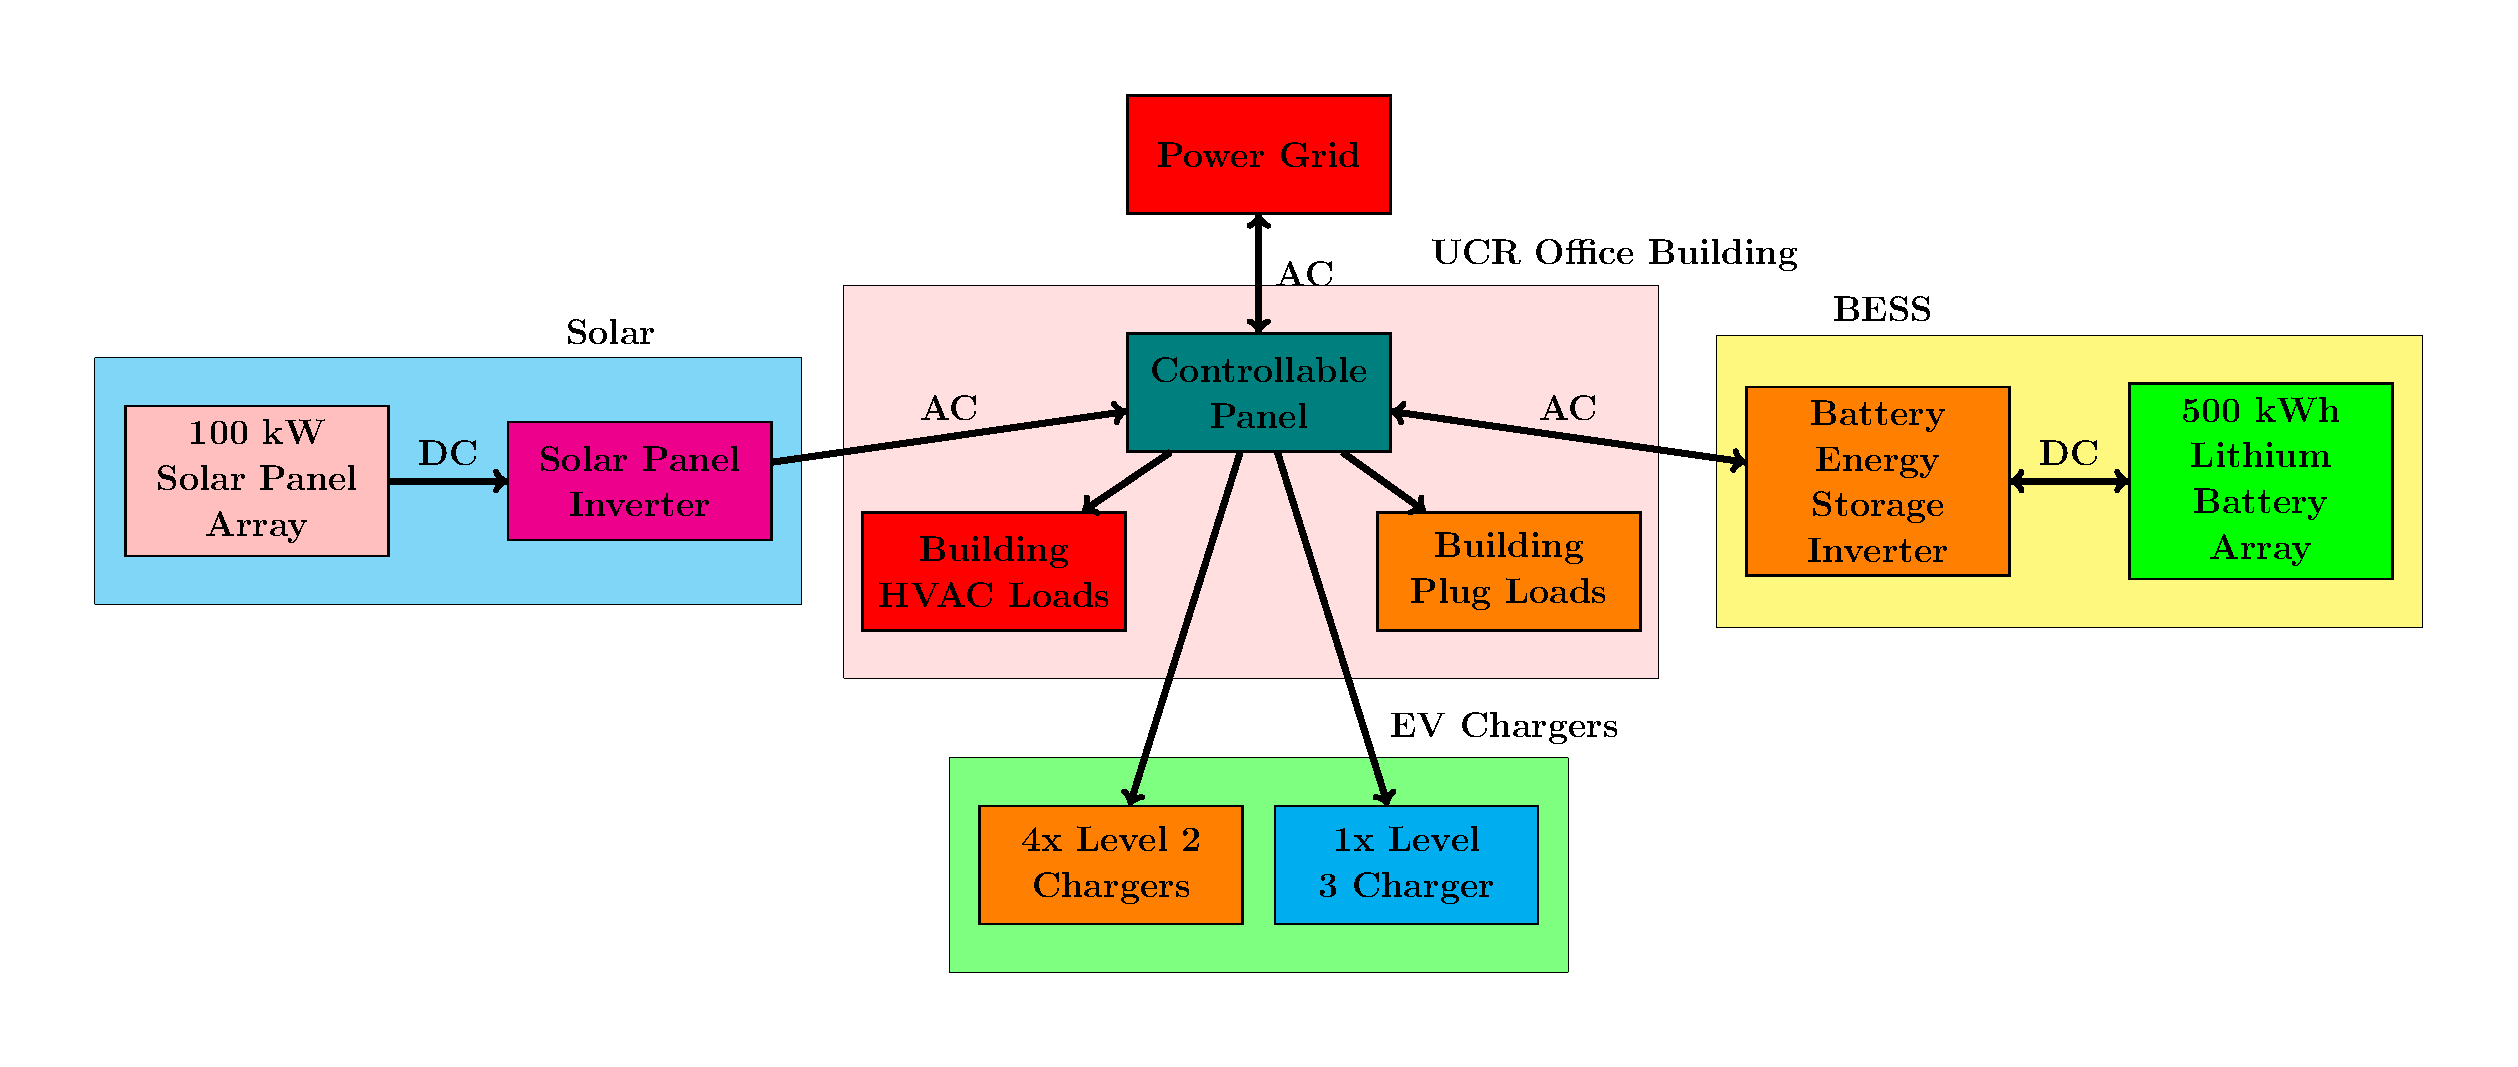
\includegraphics[width=0.88\linewidth]{Fig/power_system_setup_modelica_large}
			\caption{Microgrid Architecture of our Case Study Example BESS: Battery Energy Storage System}
			\label{fig:powersystemsetupfull}
		\end{figure}
	\end{frame}

\section{Results}	
		
		\begin{frame}
			\frametitle{Results}
			\begin{itemize}
				\item The charging setup is modified in OpenModelica for different layouts and scenarios
				\item The scenarios are described in Table \ref{tab:scenarios}
			\end{itemize}
			
			\begin{table}
				\caption{Simulated Scenarios of the UCR Microgrid using Different Layouts and Electric Pricing Structures}
				\large
				\begin{tabularx}{\linewidth}{l | l}
\toprule
 Scenario &  \\
\midrule
		1  & Standard Building with no EV Chargers\\
        2 & Standard Building with Level 2 and Level 3 Charging\\
        3 & Microgrid Building with 100 kW Solar, 500 kWh BESS, No EV Charging \\
        4 & Microgrid Building with 100 kW Solar, 100 kWh BESS, Level 2, and Level 3 Charging\\
        5 & Microgrid Building with 100 kW Solar, 250 kWh BESS, Level 2, and Level 3 Charging\\
        6 & Microgrid Building with 100 kW Solar, 500 kWh BESS, Level 2, and Level 3 Charging\\
        7 & Microgrid Building with 100 kW Solar, 1 MWh BESS, Level 2, and Level 3 Charging\\
        8 & Microgrid Building with 100 kW Solar, 1 MWh BESS, Level 2, and Level 3 Charging\\
\bottomrule
\end{tabularx}

				\label{tab:scenarios}
			\end{table}
		\end{frame}
		
			\begin{frame}
				\frametitle{Results}
				\begin{table}
					\caption{Microgrid Utility Prices and CO\textsubscript{2} Emissions Output under Different Pricing Scenarios and Pricing Structures}
					\centering
					\large
					\input{Table/kw_kwh_CO2_run_4.tex}
					\label{tab:emissions}
				\end{table}
		\end{frame}

		\begin{frame}
			\frametitle{Results}
			\begin{figure}
				\centering
				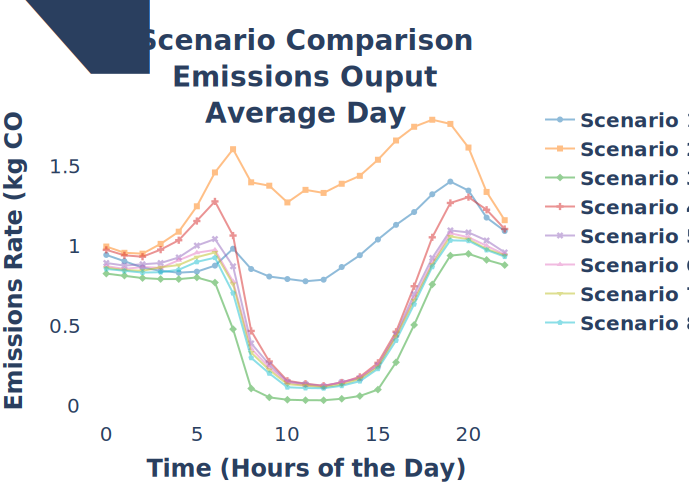
\includegraphics[width=0.7\linewidth]{Fig/emissions_scenario_comparison_run_3_large_font}
				\caption{Microgrid CO\textsubscript{2} Emissions Outputs Averages During Times of Day: Adding a microgrid significantly reduces CO\textsubscript{2} Emissions compared to the non-microgrid scenarios 1 and 2.}
				\label{fig:emissionsscenariocomparison}
			\end{figure}
		\end{frame}
	
		\begin{frame}
			\frametitle{Results}
			\begin{figure}
				\centering
				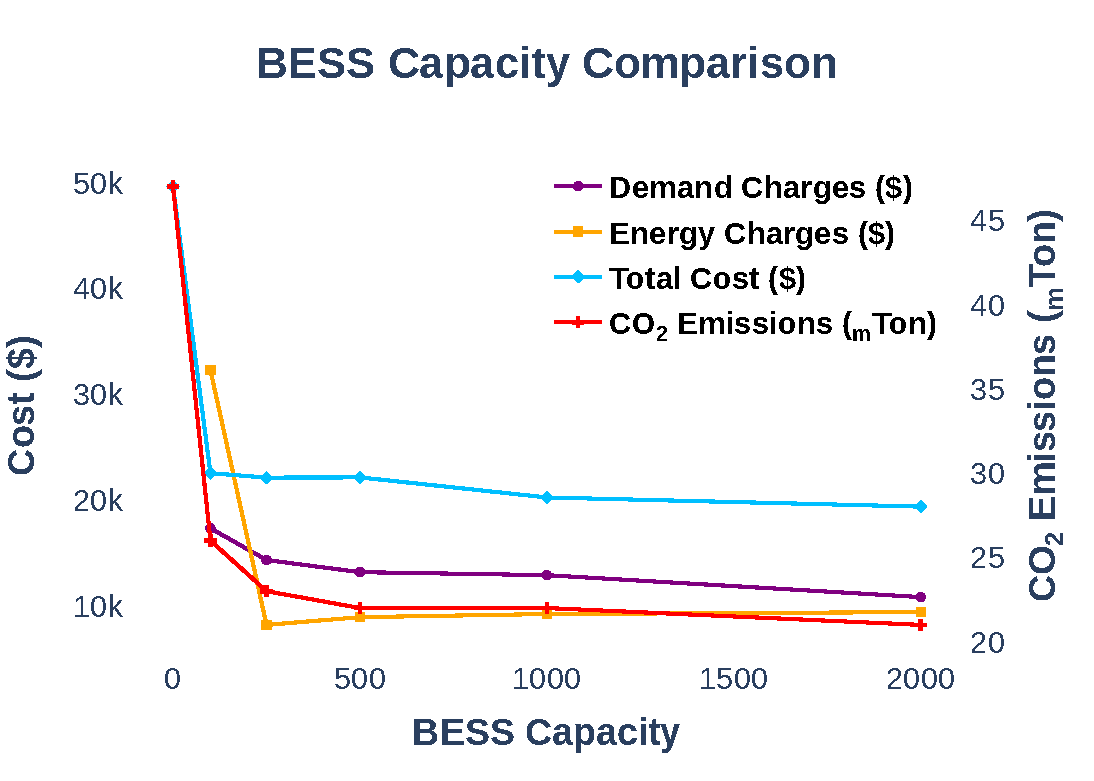
\includegraphics[width=0.7\linewidth]{Fig/bess_capacity_comparison_large_font}
				\caption{Cost and CO\textsubscript{2} Emissions for Different Battery Capacities: A BESS capacity of 250 -500 kWh is ideal for lowering costs and CO\textsubscript{2} emissions without with less diminishing returns in savings. }
				\label{fig:besscapacitycomparison}
			\end{figure}
		\end{frame}
		
\section{Conclusions and Future Work}		
		
		\begin{frame}
			\frametitle{Conclusions and Future Work}
			\begin{itemize} \Large
				\item Transportation-microgrids offer significant economic and environmental benefits
					\begin{itemize} \large
						\item Estimated annual savings of \$8,000-\$10,000 compared to conventional systems
						\item Annual savings of \$27,000-\$29,000 compared to buildings with EV chargers but no microgrid
						\item 24\% - 38\% reduction in CO\textsubscript{2} emissions compared to conventional buildings
						\item 45\% - 55\% reduction in CO\textsubscript{2} emissions compared to buildings with EV chargers and no microgrid
					\end{itemize}
				\item Increased battery capacity does not guarantee improved performance
					\begin{itemize} \large
						\item Increased capacity improves performance but not proportionally to the cost
						\item Large capacity needed for challenging situations may not be cost-effective 
					\end{itemize}
				\item 15 kW demand price floor discourages zero net load
					\begin{itemize} \large
						\item Discourages zero net load in peak shaving setups, increasing CO\textsubscript{2} emissions
					\end{itemize}
				\item Future Work
					\begin{itemize} \large
						\item Optimizing electric costs and CO\textsubscript{2} emissions through throttling charging, maximizing solar energy use, and minimizing grid draw during peak CO\textsubscript{2} emissions times
						\item Assessing the impact of California's new net energy metering policy
					\end{itemize}
			\end{itemize}
		\end{frame}
	
	\begin{frame}
		\frametitle{\null}
		\centering
		\Huge
		Questions?
	\end{frame}
	
	\begin{frame}
		\frametitle{\null}
		\centering
		\Huge
		Thank You
	\end{frame}
\end{document}
